L% MLSys 2025 paper skeleton (reset)
\documentclass{article}

% Recommended packages
\usepackage{microtype}
\usepackage{graphicx}
\usepackage{subfigure}
\usepackage{amsmath,amssymb}
\usepackage{booktabs}

% MLSys style
\usepackage{mlsys2025}

% Running title (short)
\mlsystitlerunning{Theoretical grounds for popularity bias in two-tower models}

\begin{document}

\twocolumn[
\mlsystitle{Theoretical grounds for popularity bias in two-tower models trained with cosine-based loss}

% Keywords are optional
\mlsyskeywords{Representation learning, Two-tower models, Embedding norms}

\vskip 0.1in
\begin{abstract}
    Two-tower models trained with contrastive loss may exhibit popularity bias, observed as a positive correlation between item frequency and its embedding norm that inflates dot-product scores at ranking time. This phenomenon is due to specific properties of loss and encoder architecture. Using analysis of encoder parameters’ updates, I identify sufficient conditions under which embedding updates are provably orthogonal to the current embedding and hence monotonically increase its norm. My theory yields explicit guarantees for the emergence of popularity bias in practical two-tower setups (InfoNCE/cosine-based loss, asymmetric two-tower architecture) and corrects a common misconception in prior works that orthogonality of the gradient alone implies norm inflation for deep encoders.  Empirical studies support the theory via geometry-first investigation: configurations that satisfy these premises exhibit strictly orthogonal embedding movements and a robust statistically significant frequency–norm coupling, whereas violations of any premise break orthogonality and yield non-systematic, noisy update trajectories. The results provide theoretical grounds for popularity bias in cosine-trained two-tower models and show when it should be expected in production systems.
\end{abstract}
]

% Author and affiliation footnote (auto-handled by style in review mode)
\printAffiliationsAndNotice{\mlsysEqualContribution}

% Introduction
\section{Introduction}
Two-tower architectures are the de facto standard for large-scale retrieval and recommendation. Their efficiency stems from decoupling the user and item encoders and scoring by a simple similarity, which enables precomputation, approximate nearest-neighbor search, and low-latency serving at web-scale. Yet the role of embedding magnitudes in training and ranking remains under-characterized: empirical observations vary across systems, and theory has not reached consensus on when and why norms change under different objectives and optimizers.

From the definition of cosine similarity, \(\cos(q,k)=\langle q,k\rangle/(\|q\|\,\|k\|)\), the normalization appears to cancel the effect of magnitudes, so objectives that couple the left and right encoder embeddings only through cosine similarity are expected to be insensitive to embedding norms. A competing line of analysis argues that for cosine-based losses the gradient \(\nabla_{q}\,\mathcal{L}\) is orthogonal to \(q\), and therefore any gradient step must increase \(\|q\|\), often extrapolated to deep encoders. Both perspectives ignore how parameter updates propagate through the encoder and fail to state the algorithmic and architectural conditions under which norm growth necessarily occurs.

I replace black-box reasoning with an update-level analysis. I track how parameter updates map to item-embedding displacements and prove that, under explicit and testable premises—the item encoder is linear in its parameters with non-shared per-item parameters; the item side is trained by plain SGD; and the loss uses the item embedding only via cosine similarities—each step moves the embedding orthogonally to its current value and thus monotonically increases its norm. From this, I derive a frequency--norm law: expected radial growth increases with item sampling frequency and diminishes with the current norm, yielding a concrete mechanism for popularity bias in asymmetric two-tower systems.

The analysis also delineates the limits of claims that ``gradient orthogonality implies norm inflation'' for deep encoders. Orthogonality of the output gradient is insufficient on its own; orthogonality of the \emph{update} follows only when the encoder's Jacobian preserves it, which holds precisely under the stated premises. Violating any premise--adding nonlinearities or parameter sharing in the item tower or optimizing dot product--breaks the guarantee and leads to non-systematic norm dynamics. My contributions are:

\begin{itemize}
    \item \textbf{Explanation of sufficient conditions for orthogonality of embedding updates.} I prove that embeddings move orthogonally under the following premises: (A1) the item encoder is linear in its parameters; (A2) per-item parameters are not shared; (A3) the loss depends on the item only via cosine; and (A4) the item side is optimized by SGD without regularization. Orthogonality breaks if any premise is violated.
    \item \textbf{Explanation of why orthogonality of embedding updates implies norm growth.} Using \emph{coupling} probabilistic technique I prove that orthogonal movement makes more popular item have systematically bigger embedding norm.  
    \item \textbf{Clarification of prior claims in the literature.} I re-examine claims from studies on similar topic [1][2][3] and argue that gradient update affects the model parameters, not its output itself.
    \item \textbf{Common two-tower configurations that produce popularity bias.} Given complexity of modern architectures, the guarantees on popularity bias can still hold in production-style two-tower setups if item tower meet premises.
\end{itemize}

All my claims are supported by experimental results.

\paragraph{Scope and implications.} TODO

\paragraph{Paper organization.} TODO
\section{Sufficient Conditions for Orthogonality of Embedding Updates}

\section{Одна формула, на которой строится весь анализ}
Рассматриваем двухбашенную архитектуру с левым и правым энкодерами. Обозначим для любого примера батча градиент лосса по выходу энкодера как \(g_j = \partial \mathcal{L}/\partial q_j\), а Якобиан выхода по параметрам энкодера как \(J_j = \partial q_j/\partial \theta\). Тогда градиент по параметрам и шаг SGD задают приращение параметров \(\Delta\theta\), а линейная аппроксимация первого порядка даёт приращение выхода для конкретного примера \(i\):
\[
\Delta q_i = J_i\,\Delta\theta = -\eta\sum_j J_i J_j^{\top} g_j.
\]
Эта формула служит отправной точкой дальнейшего анализа условий, когда нормa \(\|q_i\|\) коррелирует с популярностью объекта.

\subsection{Interim Focus: Parameter-Linear Encoders}

The equation developed above is a \emph{linear approximation} of the embedding dynamics during training. For parameter-linear encoders this linearization is exact: for each example $i$ the map from parameters to the output satisfies $q_i(\theta)=J_i\,\theta$, and hence equation \eqref{eq:starting-formula} holds without approximation.

For non-linear encoders, the relation $\Delta q_i \approx J_i\,\Delta\theta$ remains accurate under sufficiently small learning rates. I postpone a full treatment of the additional constraints imposed by non-linear architecture to Section~\ref{sec:beyond-linear} (\emph{Beyond linear encoders}).


\subsection{What Is a Parameter-Linear Encoder}

For notation, let
\( q(\theta, x_i) := q_i \) 
denote the encoder output with parameters $\theta$ given input $x_i$ (e.g., categorical feature or feature vector for example $i$), and
\( J(x_i) := J_i \) 
the Jacobian $\partial q(\theta, x_i)/\partial\theta$.

The encoder is \emph{parameter-linear} if its output for any input example $i$ can be written in the exact linear form
\begin{align}
q(\theta, x_i) = J(x_i)\,\theta
\end{align}
where $J(x_i)$ does not depend on $\theta$ and is therefore constant over the parameter space.

Consequently, if the encoder is parameter-linear, then equation \eqref{eq:starting-formula} holds without approximation.

Examples are deferred to Appendix~\ref{app:encoders}: a single embedding layer (Appendix~\ref{app:embed}) and a single linear layer without bias (Appendix~\ref{app:linear}) are parameter-linear; by contrast, two consecutive linear layers without bias are not (Appendix~\ref{app:two-linear}).
\subsection{For Some Linear Encoders, the Embedding Update Is Collinear with the Loss Gradient}

Drawing on equation \eqref{eq:starting-formula}, I now characterize when the embedding displacement is collinear with the output gradient: 
\begin{align}
\Delta q_{i} \,=\, J_{i}\,\Delta\theta \,=\, -\eta\,\sum_{j} J_{i}\,J_{j}^{\!\top}\,g_{j} \label{eq:collinearity-master}
\end{align}

Collinearity of the loss gradient $g_i = \nabla_{q_i}\mathcal{L}$ with the embedding update $\Delta q_i$ arises when the pairwise Jacobian products satisfy the following operator conditions:
\begin{description}
\item[(i)] $J_{i}J_{j}^{\!\top}=0$ for $j\neq i$ (all non-$i$ terms vanish in the batch sum, thus other gradients $g_j$ do not affect $\Delta q_i$);
\item[(ii)] $J_{i}J_{i}^{\!\top}=\alpha_i I_d$ for some scalar $\alpha_i$ ($J_{i}J_{i}^{\!\top}g_i=\alpha_i g_i$, i.e., the operator rescales but does not rotate $g_i$).
\end{description}
Under (i)–(ii) the sum in \eqref{eq:collinearity-master} reduces to
\begin{align}
\Delta q_i \,=\, -\eta\,\alpha_i\, g_i,
\end{align}
that is, the update is a scalar multiple of $g_i$.

A concise way to view this requirement is parameter separability: \emph{each distinct input $x_i$ must own a non–shared parameter row} so that perturbations tied to other inputs do not enter $\Delta q_i$.

\paragraph{Single embedding layer.}
For a single embedding layer (Appendix~\ref{app:embed}),
\begin{align}
J_{i}J_{j}^{\!\top} \,=\, \begin{cases}
I_d, & x_i = x_j, \\
0, & \text{otherwise.}
\end{cases} \label{eq:JJ-embed}
\end{align}
If $c_i$ denotes the number of occurrences of $x_i$ in the batch, substituting \eqref{eq:JJ-embed} into \eqref{eq:collinearity-master} yields
\begin{align}
\Delta q_i \,=\, -\eta\,c_i\,g_i.
\end{align}
Hence the update is strictly collinear with $g_i$.

\paragraph{Single linear layer without bias.}
For a single linear layer (Appendix~\ref{app:linear}),
\begin{align}
J_{i}J_{j}^{\!\top} \,=\, (x_i^{\!\top} x_j)\, I_d. \label{eq:JJ-linear}
\end{align}
Therefore,
\begin{align}
\Delta q_i \,=\, -\eta\,c_i\,\|x_i\|^2\,g_i -\; \eta\,\sum_{j\neq i}(x_i^{\!\top}x_j)\,g_j
\end{align}
If the distinct inputs are pairwise orthogonal (e.g., one-hot features or, more generally, $x_i^{\!\top}x_j=0$ for $i\neq j$), the cross-terms vanish and the self-terms aggregate over the $c_i$ occurrences of $x_i$ in the batch,
\begin{align}
\Delta q_i \,=\, -\eta\,c_i\,\|x_i\|^2\,g_i,
\end{align}
which is again collinear with $g_i$.

These cases illustrate a general principle: whenever $J_{i}J_{j}^{\!\top}$ is diagonal in the sense of \(J_{i}J_{j}^{\!\top} = \alpha_{ij} I_d\) with $\alpha_{ij}=0$ for $j\neq i$, the embedding update aligns with the output gradient. In particular, with one-hot features (orthogonal inputs), a bias-free linear layer and an embedding lookup are equivalent mappings up to implementation (matrix multiplication versus table lookup).

\paragraph{Beyond linear encoders.}\label{sec:beyond-linear}
For encoders which are not parameter-linear, I am not aware of natural conditions under which (i) and (ii) hold, even when the first-order approximation $\Delta q_i \approx J_i\,\Delta\theta$ is accurate (e.g., under small learning rates). In practice, non-linearity perturbs $J_i$ in an input- and parameter-dependent way that breaks both the cross-term annihilation (i) and the isotropy (ii). See Figure 1 for a mind map of conditions for collinearity.

\subsection{For Any Cosine-Based Loss, the Output Gradient Is Orthogonal to the Encoder Output}

Let the embedding $q$ produced by the encoder participate in the loss only via cosine similarities with other embeddings generated by the two-tower model. Then the loss can be written as
\begin{align}
\mathcal L \,=\, F\bigl(\cos(q,k_1),\dots,\cos(q,k_r)\bigr).
\end{align}
And its gradient with respect to $q$ is
\begin{align}
\nabla_q\mathcal L \,=\, \sum_{s=1}^{r} \frac{\partial F}{\partial \cos(q,k_s)}\, \nabla_q \cos(q,k_s). \label{eq:grad-cos-loss}
\end{align}
Here the derivative of the loss with respect to a cosine is a scalar. I can say that the loss gradient with respect to $q$ is orthogonal to $q$ if
\begin{align}
\langle q,\nabla_q\mathcal L \rangle \,=\, 0.
\end{align}
Therefore,
\begin{equation}
\begin{aligned}
\langle q,\nabla_q\mathcal L \rangle 
&= \sum_{s=1}^{r} \frac{\partial F}{\partial \cos(q,k_s)}\, \langle q,\nabla_q \cos(q,k_s) \rangle \\
&= 0.
\end{aligned}
\end{equation}
Here I used lemma in Appendix~\ref{app:cos-orth-lemma}, which states that $\langle q, \nabla_q \cos(q,\ast) \rangle = 0$.
Hence $q_i \perp g_i$ for any cosine loss. Consequently, 
\begin{equation}
\begin{aligned}
\textit{if } \Delta q_i \parallel g_i \textit{, then } q_i \perp \Delta q_i, \label{eq:ort-move-proof}
\end{aligned}
\end{equation}
which implies that during training the embedding moves orthogonally:

\begin{figure}[!htbp]
\centering
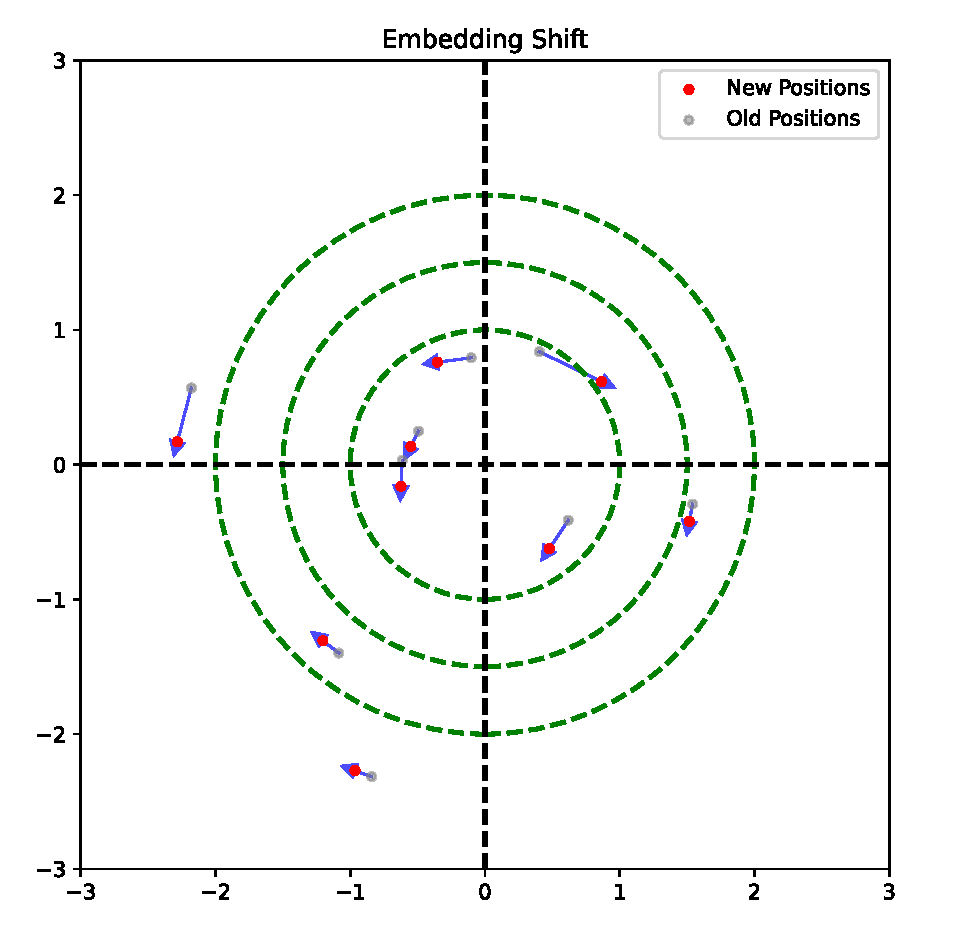
\includegraphics[width=.95\columnwidth]{../draft_materials/figure_2_paper.pdf}
\caption{Orthogonal movement during training.}
\label{fig:cos-orth}
\end{figure}


\subsection{Proposition: When Embeddings Move Orthogonally}

If, in a two-tower model, the encoder satisfies the following four conditions simultaneously:
\begin{enumerate}
  \item optimization uses SGD without momentum and without regularization,
  \item the encoder is linear in its parameters (parameter-linear),
  \item each distinct input has a dedicated, non-shared parameter row (no overlap across inputs),
  \item the loss gradient with respect to the encoder output (the embedding) is orthogonal to that output,
\end{enumerate}

then it can be proved analytically that, during training, the embedding moves orthogonally, i.e., tangentially to the hypersphere on which it located at the previous step.

\subsection{Related work on orthogonal movement}

In \emph{NormFace: L2 Hypersphere Embedding for Face Verification} (\textasciitilde930 citations) a new way to train deep encoders is proposed. In Section~3.2 they prove that, at the model output, for $x$ and the gradient $\partial\mathcal{L}/\partial x$, orthogonality holds, after which they immediately make the logical transition \emph{``it can be inferred that after update, $\|x\|^2$ always increases''}, i.e., they implicitly assume that if the loss gradient with respect to the model output is orthogonal to the model output, then this output itself also moves orthogonally. This transition is not obvious: it switches from orthogonality of the gradient to orthogonality of the update itself.

Such orthogonality of the step is guaranteed only under a sufficiently strict set of conditions. I write these conditions explicitly and show that, when they are satisfied, embeddings do move orthogonally; outside this region the transition from orthogonality of the gradient to orthogonal motion of the embedding (and hence to monotone growth of the embedding norm) may fail. Consequently, the motivation for modifying training \emph{because the update increases the point's norm} should be treated as a qualified claim: it is true in the configurations described by my conditions, but it is not a universal basis for changing how encoders are trained—especially deeper ones.

The same critique applies to \emph{The Hidden Pitfalls of the Cosine Similarity Loss} and \emph{On the Importance of Embedding Norms in Self-Supervised Learning}. In particular, the former states that \emph{``The gradient is orthogonal to the embedding, so a step of gradient descent can only increase the embedding's magnitude''} and that \emph{``these derivations are extremely general—they hold across deep learning architectures''}, without accounting for the fact that the gradient is taken with respect to the model output rather than the parameters; it also supports the claim only by observing norm growth in experiments, without analyzing whether that growth is indeed caused by orthogonal motion of the embedding. The latter states that \emph{``Because gradient updates are orthogonal to an embedding point, they must increase the point’s norm''}, which is correct only after refining the conditions under which the embedding displacement (and not just the gradient) is orthogonal. Such a simplification can mislead the reader about the universality of the "inevitable catch-22".

It should be acknowledged that in Appendix~B they provide a qualification, stating \emph{``We optimize the cosine similarity by performing standard gradient descent on the embeddings themselves''}, which implies a shallow architecture such as an Embedding Layer; however, this architectural restriction (if intended) is fixed only in the appendix, while the main text presents the correctness of the claim \emph{``Because gradient updates are orthogonal to an embedding point, they must increase the point’s norm''} without specifying the architecture.

When the conditions above do hold, my analytic proof of orthogonal embedding motion indeed implies growth of the embedding norm (by the Pythagorean theorem). A natural question then arises: how should this growth be evaluated analytically?





\section{Key observation about embedding updates}
---

\section{What does parameter-linear encoder mean}
---

\section{Architectures that are parameter-linear}
---

\section{A non-parameter-linear counterexample}
---

\section{When is \(\Delta q_i\) aligned with \(g_i\)}
---

\section{Cosine gradients are orthogonal to outputs}
---

\section{When orthogonal motion appears}
---

\section{Relation to prior work on orthogonality}
---

\section{Norm growth and popularity}
---

\section{Mitigations}
---


\section{Experiments: Empirical Validation of Theoretical Results}
\label{sec:experiments}

To clarify scope, we do not assess recommendation quality on held-out datasets and we do not report relevance metrics (e.g., MAP@k). 
Instead, we empirically examine geometric properties of the training dynamics across encoder architectures and training designs, focusing on the orthogonality of embedding updates and the frequency–norm coupling predicted by the theory.

\subsection{Factors Under Which Embedding-Motion Orthogonality Emerges}

\textit{Dataset and protocol.} We use a small toy synthetic dataset in which personalized dependencies can be observed visually; the dataset and all scripts are available in a public GitHub repository X (link to be added). Throughout these experiments, the right (item) tower is a simple embedding layer.

\textit{Definitions.} 
Condition~1: the encoder architecture consists of either (i) a single linear layer applied to one-hot inputs, or (ii) an embedding layer. 
Condition~2: the gradient of the loss with respect to the encoder output is orthogonal to that output.

\begin{table*}[!t]
\centering
\small
\begin{tabular}{@{}cccccc@{}}
\toprule
No. & Left encoder & Loss & Cond.~1? & Cond.~2? & Orthogonal trajectory? \\
\midrule
1 & Embedding & InfoNCE (cos) & $\checkmark$ & $\checkmark$ & $\checkmark$ \\
2 & Embedding & InfoNCE (dot) & $\checkmark$ & $\times$ & $\times$ \\
3 & BERT-like & InfoNCE (cos) & $\times$ & $\checkmark$ & $\times$ \\
4 & Embedding $\to$ Linear & InfoNCE (cos) & $\times$ & $\checkmark$ & $\times$ \\
5 & Embedding (frozen) $\to$ Linear & InfoNCE (cos) & $\times$ & $\checkmark$ & $\times$ \\
6 & one-hot $\to$ Linear & InfoNCE (cos) & $\checkmark$ & $\checkmark$ & $\checkmark$ \\
7 & Embedding & $\bigl(1 - \cos(q,k)\bigr)^{2}$ & $\checkmark$ & $\checkmark$ & $\checkmark$ \\
\bottomrule
\end{tabular}
\caption{Summary of experiments probing when the left-encoder trajectory is orthogonal.}
\end{table*}

\textit{Clarifications.} In all experiments the item tower is nn.Embedding; InfoNCE denotes the contrastive softmax loss with in-batch negatives, where ``cos'' (resp., ``dot'') refers to cosine (resp., dot-product) similarity. We use vanilla SGD without momentum; alternative optimizers did not reveal additional dependence, though we will separately analyze mixed-optimizer settings (including Adam) later (see Experiment~10).

\paragraph{What happens if the encoder is nonlinear in the parameters?}
Two linear layers constitute nonlinearity with respect to the model parameters. Under such nonlinearity the analytic explanation above does not apply. Consistently, Experiment~4 shows that, unlike Experiments~1 and~6, left-encoder embeddings move in a non-orthogonal, chaotic manner.

\paragraph{What if, despite parameter linearity, the inputs to the encoder are not mutually orthogonal?}
Linearity of the encoder is not sufficient to guarantee orthogonal motion. Experiment~5 shows that embeddings produced by the left encoder move chaotically when inputs are not orthogonal. For orthogonality we require that every unique input has its own parameter row that does not overlap with others. We find only two architectures where this holds: a linear layer over one-hot vectors (Experiment~6) and an embedding layer (Experiment~1).

\paragraph{What if we change the loss?}
The outcome of Experiment~7 is consistent with the statement that the gradient of any cosine-based loss with respect to the encoder output is orthogonal to that output.

These experiments increase our confidence in the analytical conclusions about orthogonality of embedding motion.





\section{Discussion}
---


\section{Limitations}
---


\section{Conclusion}

If the following factors hold simultaneously for the item tower, then item embeddings of more popular items systematically attain larger norms than those of less popular items:
\begin{enumerate}
  \item optimization uses SGD without momentum and without regularization (the only way to guarantee strict movement defined by equations), 
  \item the encoder is linear in its parameters (parameter-linear),
  \item each distinct input has a dedicated, non-shared parameter row (no overlap across inputs),
  \item the loss gradient with respect to the encoder output (the embedding) is orthogonal to that output,
  \item the learning rate is sufficiently large (orthogonality itself does not require this; the point is to overcome the random initialization of embeddings by ensuring sufficiently large orthogonal displacement).
\end{enumerate}

This list makes explicit how many requirements must be met so that embeddings move orthogonally, their norms grow monotonically, and this growth yields popularity bias. In this way, our investigation refines the takeaways of prior work by specifying exactly which factors guarantee orthogonal embedding movement. To the best of my knowledge, these aspects have not been articulated in the literature on representation learning with cosine–based objectives.

An important observation is that, although these strict conditions restrict the encoder architecture for which we can provide analytic guarantees of popularity bias, modern two–tower systems contain two independent encoders. Even if one of them is a complex deep model with a complicated training dynamics, the other one—provided its architecture is sufficiently primitive—already guarantees the emergence of the phenomenon when trained with a cosine loss. This observation allows us to transfer the present mathematical guarantees to practical systems where, for example, the user tower is a transformer over his history with a sophisticated optimizer, while the item tower is a simple embedding layer trained with SGD without momentum and without regularization.

Thus, we revisited the academic stance on the geometry of embedding movement under cosine–based training. Although orthogonality of movement (and the resulting popularity bias) requires strict constraints on the encoder architecture, popular two–tower designs can still employ a deliberately simple item tower that provably preserves orthogonal movement and leads to popularity bias. 
This may be critical for downstream ranking tasks -- for example, index search based on dot products -- if this property of the training process is not taken into account.


% References
\bibliography{references}
\bibliographystyle{mlsys2025}

\appendix
\section{Appendix}
---


\end{document}
